\chapter{Parallel Computation in Statistics/Data Mining}
\label{chap:stat}

How did the word {\it statistics} get supplanted by {\it data mining}?
In a word, it is a matter of scale.

In the old days of statistics, a data set of 300 observations on 3 or 4
variables was considered large.  Today, the widespread use of computers
and the Web yield data sets with numbers of observations that are easily
in the tens of thousands range, and in a number of cases even tens of
millions.  The numbers of variables can also be in the thousands or
more.

In addition, the methods have become much more combinatorial in nature.
In a classification problem, for instance, the old discriminant analysis
involved only matrix computation, whereas a nearest-neighbor analysis
requires far more computer cycles to complete.

In short, this calls for parallel methods of computation.

\section{Itemset Analysis}

\subsection{What Is It?}

The term {\bf data mining} is a buzzword, but all it means is the
process of finding relationships among a set of variables.  In other
words, it would seem to simply be a good old-fashioned statistics
problem.

Well, in fact it {\it is} simply a statistics problem---but writ large,
as mentioned earlier.

{\bf Major, Major Warning:}  With so many variables, the chances of
picking up spurious relations between variables is large.  And although
many books and tutorials on data mining will at least pay lip service to
this issue (referring to it as {\bf overfitting}), they don't emphasize
it enough.\footnote{Some writers recommend splitting one's data into a
{\bf training set}, which is used to discover relationships, and a {\bf
validation set}, which is used to confirm those relationships.  It's a
good idea, but overfitting can still occur even with this precaution.}

Putting the overfitting problem aside, though, by now the reader's
reaction should be, ``This calls for parallel processing,'' and he/she
is correct.  Here we'll look at parallelizing a particular problem,
called {\bf itemset analysis}, the most famous example of which is the
{\bf market basket problem}:

\subsection{The Market Basket Problem}

Consider an online bookstore that has records of every sale on the
store's site.  Those sales may be represented as a matrix S, whose
(i,j)th element $S_{ij}$ is equal to either 1 or 0, depending on whether
the i$^{th}$ sale included book j, i = 0,1,...,s-1, j = 0,1,...,t-1.  So
each row of S represents one sale, with the 1s in that row showing which
titles were bought.  Each column of S represents one book title, with
the 1s showing which sales transactions included that book.

Let's denote the entire line of book titles by $T_0,...,T_{b-1}$.  An
{\bf itemset} is just a subset of this.  A {\bf frequent} itemset is one
which appears in many of sales transactions.  But there is more to it
than that.  The store wants to choose some books for special ads, of the
form ``We see you bought books X and Y.  We think you may be interested
in Z.''

Though we are using marketing as a running example here (which is the
typical way that this subject is introduced), we will usually just refer
to ``items'' instead of books, and to ``database records'' rather than
sales transactions.

We have the following terminology:

\begin{itemize}

\item An {\bf association rule} $I \rightarrow J$ is simply an ordered
pair of disjoint itemsets I and J.

\item The {\bf support} of an an association rule $I \rightarrow J$ is
the proportion of records which include both I and J.

\item The {\bf confidence} of an association rule $I \rightarrow J$ is
the proportion of records which include J, {\it among those records
which include I}.

\end{itemize}

Note that in probability terms, the support is basically P(I and J)
while the confidence is P(J$|$I).  If the confidence is high in the book
example, it means that buyers of the books in set I also tend to buy
those in J.  But this information is not very useful if the support is
low, because it means that the combination occurs so rarely that it may
not be worth our time to deal with it.

So, the user---let's call him/her the ``data miner''---will first set
thresholds for support and confidence, and then set out to find all
association rules for which support and confidence exceed their
respective thresholds.

\subsection{Serial Algorithms}

Various algorithms have been developed to find frequent itemsets and
association rules.  The most famous one for the former task is the {\bf
Apriori} algorithm.  Even it has many forms.  We will discuss one of the
simplest forms here.

The algorithm is basically a breadth-first tree search.  At the root we
find the frequent 1-item itemsets.  In the online bookstore, for
instance, this would mean finding all individual books that appear in at
least r of our sales transaction records, where r is our threshold.

At the second level, we find the frequent 2-item itemsets, e.g. all
pairs of books that appear in at least r sales records, and so on.
After we finish with level i, we then generate new candidate itemsets of
size i+1 from the frequent itemsets we found of size i.

The key point in the latter operation is that if an itemset is not
frequent, i.e. has support less than the threshold, then adding further
items to it will make it even less frequent.  That itemset is then
pruned from the tree, and the branch ends.

Here is the pseudocode:

\begin{tabbing}
set $F_1$ to the set of 1-item itemsets whose support exceeds the
threshold \\
for \=  i = 2 to b \\
  \> $F_{i} = \phi$ \\
  \> for \= each I in $F_{i-1}$ \\
  \> \> for \= each K in $F_1$ \\
  \> \> \> $Q = I \cup K$ \\
  \> \> \> if \= support(Q) exceeds support threshold \\
  \> \> \> \> add Q to $F_{i}$ \\
  \> if $F_{i}$ is empty break \\
return $\cup_i F_i$
\end{tabbing}

In other words, we are building up the itemsets of size i from those of
size i-1, adding all possible choices of one element to each of the
latter.

Again, there are many refinements of this, which shave off work to be
done and thus increase speed.  For example, we should avoid checking the
same itemsets twice, e.g. first \{1,2\} then \{2,1\}.  This can be
accomplished by keeping itemsets in lexicographical order.  We will not
pursue any refinements here.

\subsection{Parallelizing the Apriori Algorithm}

Clearly there is lots of opportunity for parallelizing the serial
algorithm above.  Both of the inner {\bf for} loops can be parallelized
in straightforward ways; they are ``embarrassingly parallel.''  There
are of course critical sections to worry about in the shared-memory
setting, and in the message-passing setting one must designate a manager
node in which to store the $F_i$.

However, as more and more refinements are made in the serial algorithm,
then the parallelism in this algorithm become less and less
``embarrassing.''  And things become more challenging if the storage
needs of the $F_i$, and of their associated ``accounting materials''
such as a directory showing the current tree structure (done via
hash trees), become greater than what can be stored in the memory of one
node, say in the message-passing case.

In other words, parallelizing the market basket problem can be very
challenging.  The interested reader is referred to the considerable
literature which has developed on this topic.

\section{Probability Density Estimation}

Let X denote some quantity of interest in a given population, say
people's heights.  Technically, the {\bf probability density function}
of X, typically denoted by f, is a function on the real line with the
following properties:

\begin{itemize}

\item $f(t) \geq 0$ for all t

\item for any $r < s$,

\begin{equation}
P(r < X < s) = \int_{r}^{s} f(t) ~ dt
\end{equation}

(Note that this implies that f integrates to 1.)

\end{itemize}

This seems abstract, but it's really very simple:  Say we have data on
X, n sample values $X_1,...,X_n$, and we plot a histogram from this
data.  Then {\it f is what the histogram is estimating}.  If we have
more and more data, the histogram gets closer and closer to the true
f.\footnote{The histogram must be scaled to have total area 1.  Most
statistical programs have options for this.}

So, how do we estimate f, and how do we use parallel computing to reduce
the time needed?

\subsection{Kernel-Based Density Estimation}

Histogram computation breaks the real down into intervals, and then
counts how many $X_i$ fall into each interval.  This is fine as a crude
method, but one can do better.

No matter what the interval width is, the histogram will consist of a
bunch of rectanges, rather than a smooth curve.  This problem basically
stems from a lack of weighting on the data.

For example, suppose we are estimating f(25.8), and suppose our
histogram interval is [24.0,26.0], with 54 points falling into that
interval.  Intuitively, we can do better if we give the points closer to
25.8 more weight.

One way to do this is called {\bf kernel-based} density estimation,
which for instance in R is handled by the function {\bf density()}.

We need a set of weights, more precisely a weight function k, called the
{\bf kernel}.  Any nonnegative function which integrates to 1---i.e. a
density function in its own right---will work.  Typically k is taken to
be the Gaussian or normal density function,

\begin{equation}
\label{gaussk}
k(u) = \frac{1}{\sqrt{2 \pi}} e^{-0.5u^2}
\end{equation}

Our estimator is then

\begin{equation}
\label{kernelest}
\widehat{f}(t) = \frac{1}{nh} \sum_{i=1}^{n} k \left ( \frac{t-X_i}{h} \right )
\end{equation}

In statistics, it is customary to use the $\ \widehat{}$ symbol
(pronounced ``hat'') to mean ``estimate of.''  Here $\ \widehat{f}$
means the estimate of f.

Note carefully that we are estimating an entire function!  There are
infinitely many possible values of t, thus infinitely many values of
f(t) to be estimated.  This is reflected in (\ref{kernelest}), as
$\widehat{f}(t)$ does indeed give a (potentially) different value for
each t.

Here h, called the {\it bandwidth}, is playing a role analogous to the
interval width in the case of histograms.  We must choose the value of
h, just like for a histogram we must choose the bin width.\footnote{Some
statistical programs will choose default values, based on theory.}

Again, this looks very abstract, but all it is doing is assigning
weights to the data.  Consider our example above in which we wish to
estimate f(25.8), i.e. t = 25.8 and suppose we choose h to be 6.0.  If
say, $X_{88}$ is 1209.1, very far as away from 25.8, we don't want this
data point to have much weight in our estimation of f(25.8).  Well, it
won't have much weight at all, because the quantity

\begin{equation}
u = \frac{25.8-88}{6}
\end{equation}

will be very large, and (\ref{gaussk}) will be tiny, as u will be way,
way out in the left tail.

Now, keep all this in perspective.  In the end, we will be plotting a
curve, {\it just like we do with a histogram}.  We simply have a more
sophiticated way to do this than plotting a histogram.  Following are
the graphs generated first by the histogram method, then by the kernel
method, on the same data:

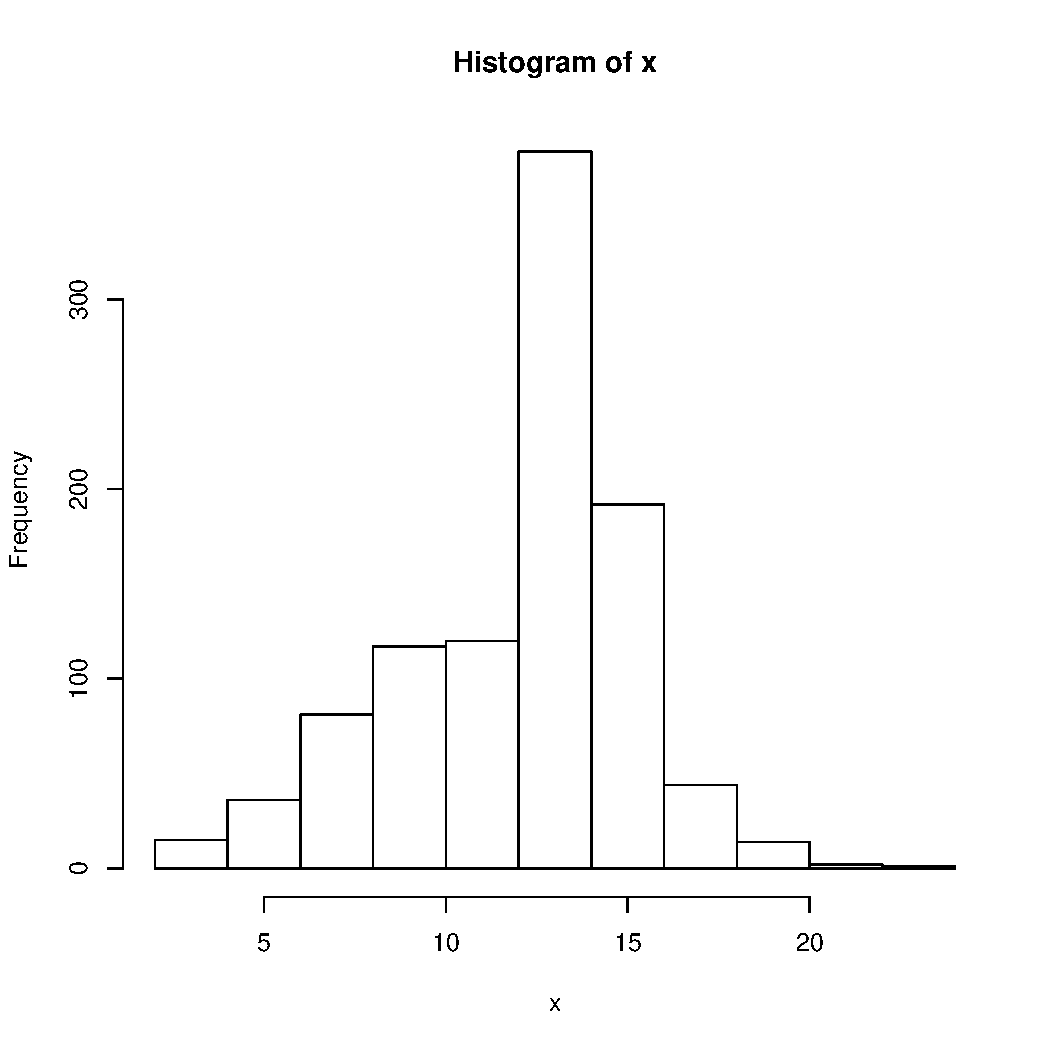
\includegraphics[width=3.0in]{Images/Hist.pdf}

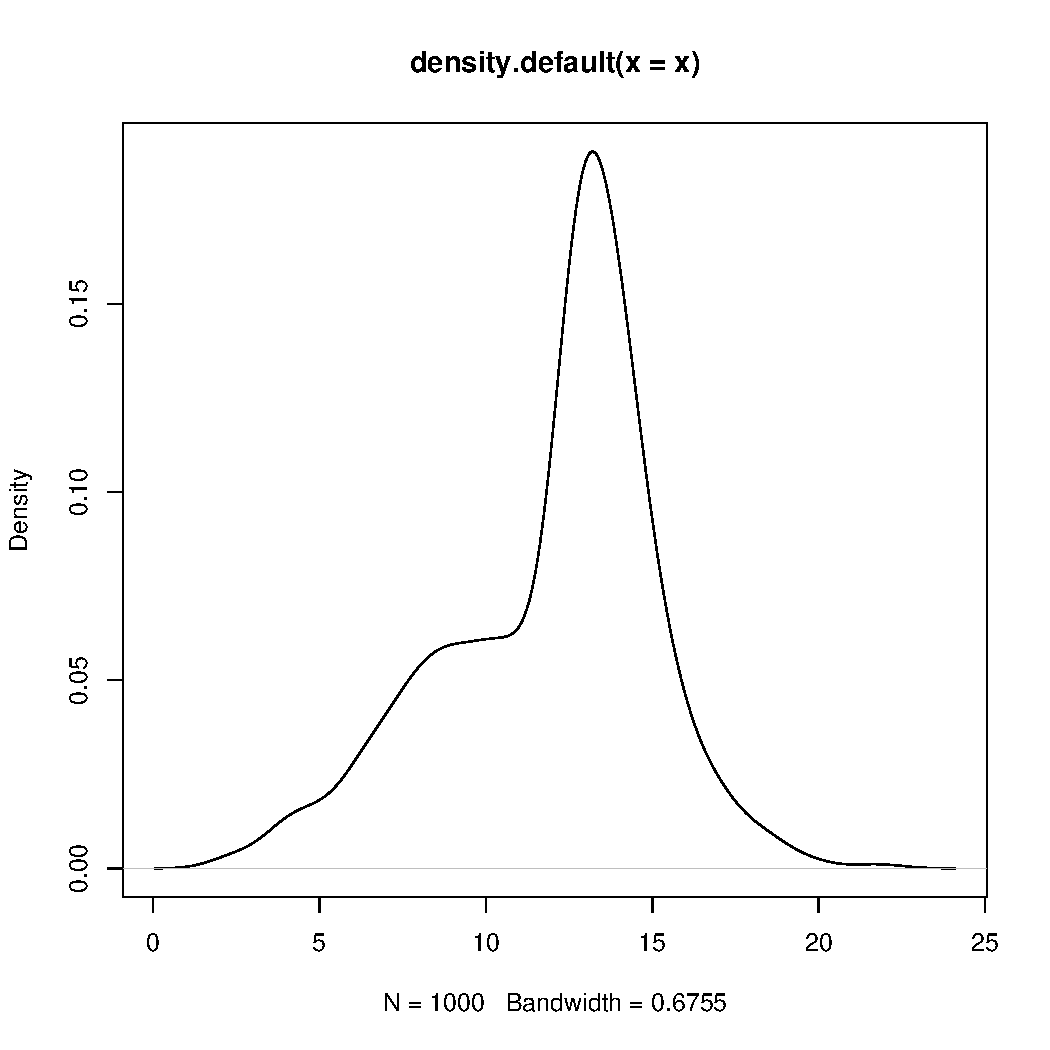
\includegraphics[width=3.0in]{Images/Kern.pdf}

% n <- 1000
% x <- vector(length=n)
% for (i in 1:n) {
%    if (runif(1) < 0.5)  {
%       x[i] <- rnorm(1,mean=10,sd=3)
%    } else x[i] <- rgamma(1,shape=2) + 12
% }
% pdf("Hist.pdf")
% hist(x)
% pdf("Kern.pdf")
% plot(density(x))

There are many ways to parallelize this computation, such as:

\begin{itemize}

\item Remember, we are going to compute (\ref{kernelest}) for many
values of t.  So, we can just have each process compute a block of those
values.

\item We may wish to try several different values of h, just as we might
try several different interval widths for a histogram.  We could have
each process compute using its own values of h.

\item It can be shown that (\ref{kernelest}) has the form of something
called a {\bf convolution}.  The theory of convolution would take us too
far afield,\footnote{

If you've seen the term before and are curious as to how this is a
convolution, read on:

Write (\ref{kernelest}) as

\begin{equation}
\label{kernelesta}
\widehat{f}(t) =
\sum_{i=1}^{n} \frac{1}{h} k \left ( \frac{t-X_i}{h} \right )
   \cdot \frac{1}{n}
\end{equation}

Now consider two artificial random variables U and V, created just for
the purpose of facilitating computation, defined as follows.

The random variable U takes on the values ih with probability $g \cdot
\frac{1}{h} k(i)$, i = -c,-c+1,...,0,1,...,c for some value of c that we
choose to cover most of the area under k, with g chosen so that the
probabilities sum to 1.  The random variable V takes on the values
$X_1,...,X_n$ (considered fixed here), with probability 1/n each.
U and V are set to be independent.

Then (g times) (\ref{kernelesta}) becomes P(U+V=t), exactly what
convolution is about, the probability mass function (or density, in the
continuous case) of a random variable arising as the sum of two
independent nonnegative random variables.} but this fact is useful
here, as the Fourier transform of a convolution can be shown to be the
product of the Fourier transforms of the two convolved
components.\footnote{Again, if you have some background in probability
and have see characteristic functions, this fact comes from the fact
that the characteristic function of the sum of two independent random
variables is equal to the product of the characteristic functions of the
two variables.} In other words, {\it this reduces the problem to that of
parallelizing Fourier transforms}---something we know how to do, from
Chapter \ref{chap:fft}.

\end{itemize}

\subsection{Histogram Computation for Images}

In image processing, histograms are used to find tallies of how many
pixels there are of each intensity.  (Note that there is thus no
interval width issue, as there is a separate ``interval'' value for each
possible intensity level.)  The serial pseudocode is:

\begin{Verbatim}[fontsize=\relsize{-2}]
for i = 1,...,numintenslevels:
   count = 0
   for row = 1,...,numrows:
      for col = 1,...,numcols:
         if image[row][col] == i: count++
   hist[i] = count
\end{Verbatim}

On the surface, this is certainly an ``embarrassingly parallel''
problem.  In OpenMP, for instance, we might have each thread handle a
block of rows of the image, i.e. parallelize the {\bf for row} loop.
In CUDA, we might have each thread handle an individual pixel, thus
parallelizing the nested {\bf for row/col} loops.

However, to make this go fast is a challenge, say in CUDA, due to issues
of what to store in shared memory, when to swap it out, etc.  A very
nice account of fine-tuning this computation in CUDA is given in {\it
Histogram Calculation in CUDA}, by Victor Podlozhnyuk of NVIDIA, 2007,
\url{http://developer.download.nvidia.com/compute/cuda/1_1/Website/projects/histogram256/doc/histogram.pdf}.
The actual code is at
\url{http://developer.download.nvidia.com/compute/cuda/sdk/website/Data-Parallel_Algorithms.html#histogram}.
A summary follows:

%   histogram64:  1-byte counts; BIN_COUNT is 64, for intensity levels
%   0-63 (data is one byte each, so ignore lower 2 bits); chooses 192 as
%   an a middle ground for efficient number of threads, THREAD_N; all
%   threads in a block share a subhistogram, but access different words
%   within it, so don't need; image data is in device global memory; the
%   portion of the subhistogram that a given thread is supposed to
%   accessed are shuffled to avoid bank conflicts; different blocks
%   handle different portions of the image, so subhistograms must be
%   merged; atomicAdd(), if available, is used to write the full
%   histogram, also in device global memory; again shuffling is done

(Much of the research into understand Podlozhnyuk's algorithm was done
by UC Davis graduate student Spencer Mathews.)

Podlozhnyuk's overall plan is to have the threads compute subhistograms
for various chunks of the image, then merge the subhistograms to create
the histogram for the entire data set.  Each thread will handle 1/k of
the image's pixels, where k is the total number of threads in the grid,
i.e. across all blocks.

In Podlozhnyuk's first cut at the problem, he maintains a separate
subhistogram for each thread.  He calls this version of the code {\bf
histogram64}.  The name stems from the fact that only 64 intensity
levels are used, i.e. the more significant 6 bits of each pixel's data
byte.  The reason for this restriction will be discussed later.

Each thread will store its subhistogram as an array of bytes; the count
of pixels that a thread finds to have intensity i will be stored in the
i$^{th}$ byte of this array.  Considering the content of a byte as an
unsigned number, that means that each thread can process only 255
pixels.

The subhistograms will be stored together in a two-dimensional array,
the j$^{th}$ being the subhistogram for thread j.  Since the
subhistograms are accessed repeatedly, we want to store this
two-dimensional array in shared memory.  (Since each pixel will be read
only once, there would be no value in storing it in shared memory, so it
is in global memory.)

The main concern is bank conflicts.  As the various threads in a block
write to the two-dimensional array, they may collide with each other,
i.e. try to write to different locations within the same bank.  But
Podlozhnyuk devised a clever way to stagger the accesses, so that in
fact there are no bank conflicts at all.

In the end, the many subhistograms within a block must be merged, and
those merged counts must in turn be merged across all blocks.  The
former operation is done again by careful ordering to avoid any bank
conflicts, and then the latter is done {\bf atomicAdd()}.

Now, why does {\bf histogram64} tabulate image intensities at only 6-bit
granularity?  It's simply a matter of resource limitations.  Podlozhnyuk
notes that NVIDIA says that for best efficiency, there should be between
128 and 256 threads per block.  He takes the middle ground, 192.  With
16K of shared memory per block, 16K/192 works out to about 85 bytes per
thread.  That eliminates computing a histogram for the full 8-bit image
data, with 256 intensity levels, which would require 256 bytes for each
thread.

Accordingly, Podlozhnyuk offers {\bf histogram256}, which refines the
process, by having one subhistogram per warp, instead of per thread.
This allows the full 8-bit data, 256 levels, to be tabulated, one word
devoted to each count, rather than just one byte.  A subhistogram is now
a table, 256 rows by 32 columns (one column for each thread in the
warp), with each table entry being 4 bytes (1 byte is not sufficient, as
32 threads are tabulating with it).

\section{Clustering}
\label{cluster}

Suppose you have data consisting of (X,Y) pairs, which when plotted look
like this:

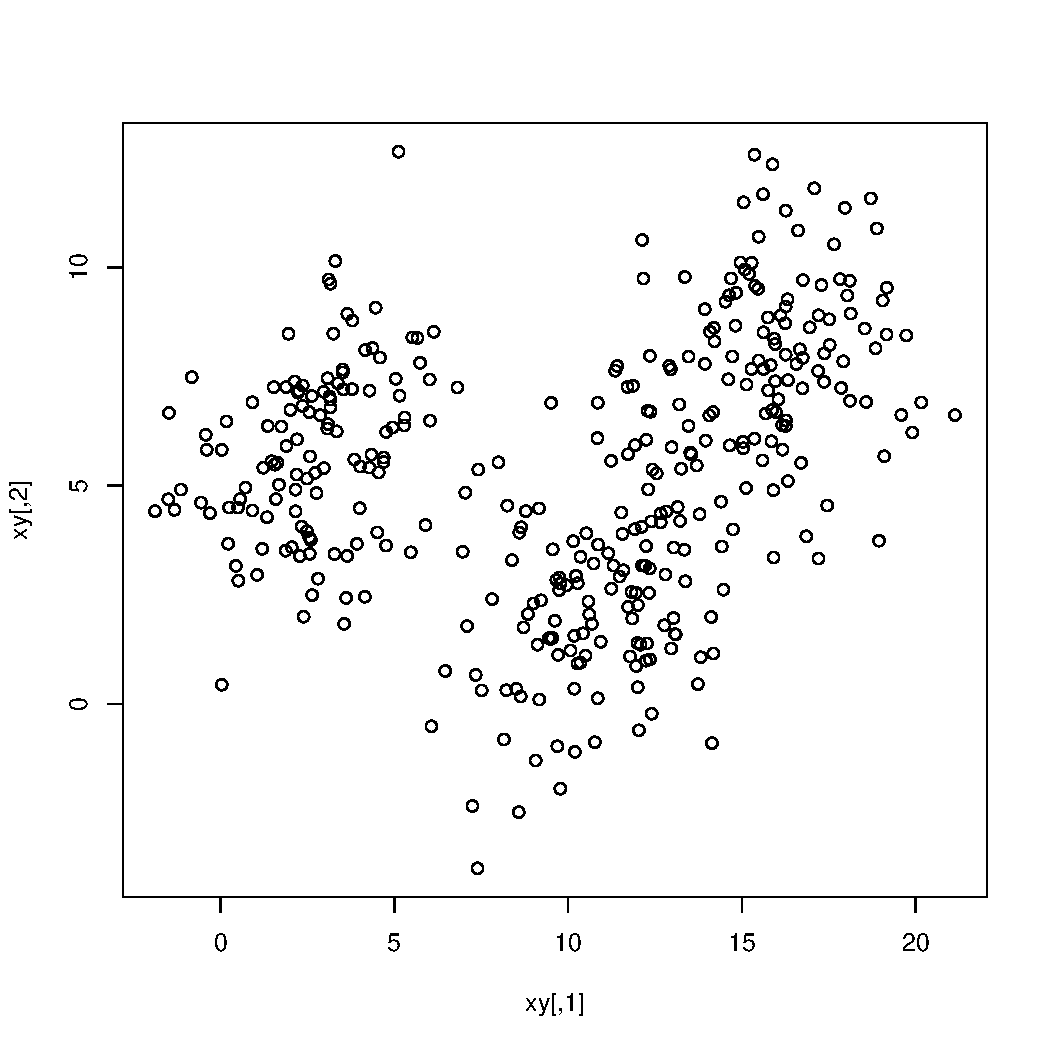
\includegraphics[width=4.0in]{Images/Scatter.pdf}

% library(MASS)
% n <- 125
% xy <- matrix(nrow=3*n,ncol=2)
% sig <- rbind(c(4,1),c(1,4))
% xy[1:n,] <- mvrnorm(n,c(3,6),sig)
% xy[(n+1):(2*n),] <- mvrnorm(n,c(16,8),sig)
% xy[(2*n+1):(3*n),] <- mvrnorm(n,c(11,2),sig)
% # pdf("Scatter.pdf")
% plot(xy)

It looks like there may be two or three groups here.  What clustering
algorithms do is to form groups, both their number and their membership,
i.e. which data points belong to which groups.  (Note carefully that
{\it there is no ``correct'' answer here.  This is merely an exploratory
data analysis tool}.)

Clustering is used is many diverse fields.  For instance, it is used in
image processing for segmentation and edge detection.

Here we have to two variables, say people's heights and weights.  In
general we have many variables, say p of them, so whatever clustering
we find will be in p-dimensional space.  No, we can't picture it very
easily of p is larger than (or even equal to) 3, but we can at least
identify membership, i.e. John and Mary are in group 1, Jenny is in
group 2, etc.  We may derive some insight from this.

There are many, many types of clustering algorithms.  Here we will
discuss the famous {\bf k-means} algorithm, developed by Prof. Jim
MacQueen of the UCLA business school.

The method couldn't be simpler.  Choose k, the number of groups you want
to form, and then run this:

\begin{Verbatim}[fontsize=\relsize{-2},numbers=left]
# form initial groups from the first k data points (or choose randomly)
for i = 1,...,k:
   group[i] = (x[i],y[i])
   center[i] = (x[i],y[i])
do:
   for j = 1,...,n:
      find the closest center[i] to (x[j],y[j])
      cl[j] = the i you got in the previous line
   for i = 1,...,k:
      group[i] = all (x[j],y[j]) such that cl[j] = i
      center[i] = average of all (x,y) in group[i]
until group memberships do not change from one iteration to the next
\end{Verbatim}

Definitions of terms:

\begin{itemize}

\item {\it Closest} means in p-dimensional space, with the usual
Euclidean distance:  The distance from $(a_1,...,a_p$ to $(b_1,...,b_p$
is

\begin{equation}
\sqrt{(b_1-a_1)^2+...+(b_p-a_p)^2}
\end{equation}

Other distance definitions could be used too, of course.

\item The {\it center} of a group is its {\bf centroid}, which is a
fancy name for taking the average value in each component of the data
points in the group.  If p = 2, for example, the center consists of the
point whose X coordinate is the average X value among members of the
group, and whose Y coordinate is the average Y value in the group.

\end{itemize}

\subsection{Example:  k-Means Clustering in R}

In terms of parallelization, again we have an embarrassingly parallel
problem.  Here's {\bf snow} code for it:

\begin{lstlisting}[numbers=left]
# snow version of k-means clustering problem

# returns distances from x to each vector in y;
# here x is a single vector and y is a bunch of them
#
# define distance between 2 points to be the sum of the absolute values
# of their componentwise differences; e.g. distance between (5,4.2) and
# (3,5.6) is 2 + 1.4 = 3.4
dst <- function(x,y) {
   tmpmat <- matrix(abs(x-y),byrow=T,ncol=length(x))  # note recycling
   rowSums(tmpmat)
}

# will check this worker's mchunk matrix against currctrs, the current
# centers of the groups, returning a matrix; row j of the matrix will
# consist of the vector sum of the points in mchunk closest to j-th
# current center, and the count of such points
findnewgrps <- function(currctrs) {
   ngrps <- nrow(currctrs)
   spacedim <- ncol(currctrs)  # what dimension space are we in?
   # set up the return matrix
   sumcounts <- matrix(rep(0,ngrps*(spacedim+1)),nrow=ngrps)
   for (i in 1:nrow(mchunk)) {
      dsts <- dst(mchunk[i,],t(currctrs))
      j <- which.min(dsts)
      sumcounts[j,] <- sumcounts[j,] + c(mchunk[i,],1)
   }
   sumcounts
}

parkm <- function(cls,m,niters,initcenters) {
   n <- nrow(m)
   spacedim <- ncol(m)  # what dimension space are we in?
   # determine which worker gets which chunk of rows of m
   options(warn=-1)
   ichunks <- split(1:n,1:length(cls))
   options(warn=0)
   # form row chunks
   mchunks <- lapply(ichunks,function(ichunk) m[ichunk,])
   mcf <- function(mchunk) mchunk <<- mchunk
   # send row chunks to workers; each chunk will be a global variable at
   # the worker, named mchunk
   invisible(clusterApply(cls,mchunks,mcf))
   # send dst() to workers
   clusterExport(cls,"dst")
   # start iterations
   centers <- initcenters
   for (i in 1:niters) {
      sumcounts <- clusterCall(cls,findnewgrps,centers)
      tmp <- Reduce("+",sumcounts)
      centers <- tmp[,1:spacedim] / tmp[,spacedim+1]
      # if a group is empty, let's set its center to 0s
      centers[is.nan(centers)] <- 0
   }
   centers
}
\end{lstlisting}



\section{Principal Component Analysis (PCA)}
\label{pca}

Consider data consisting of (X,Y) pairs as we saw in Section
\ref{cluster}.  Suppose X and Y are highly correlated with each other.
Then for some constants c and d,

\begin{equation}
\label{onedim}
Y \approx c + d X
\end{equation}

Then in a sense there is really just one random variable here, as the
second is nearly equal to some linear combination of the first.  The
second provides us with almost no new information, once we have the
first.  In other words, even though the vector (X,Y) roams in {\it
two}-dimensional space, it usually sticks close to a {\it
one}-dimensional object, namely the line (\ref{onedim}).

Now think again of p variables.  It may be the case that there exist r
$<$ p variables, consisting of linear combinations of the p variables,
that carry most of the information of the full set of p variables.  If r
is much less than p, we would prefer to work with those r variables.
In data mining, this is called {\bf dimension reduction}.

It can be shown that we can find these r variables by finding the r
eigenvectors corresponding to the r largest eigenvalues of a certain
matrix.  So again we have a matrix formulation, and thus parallelizing
the problem can be done easily by using methods for parallel matrix
operations.  We discussed parallel eigenvector algorithms in Section
\ref{eigen}.

\section{Monte Carlo Simulation}

Monte Carlo simulation is typically (though not always) used to find
probabilistic quantities such as probabilities and expected values.
Consider a simple example problem:

\begin{quote}

An urn contains blue, yellow and green marbles, in numbers 5, 12 and 13,
respectively.  We choose 6 marbles at random.  What is the probability
that we get more yellow marbles than than green and more green than
blue?

\end{quote}

We could find the approximate answer by simulation:

\begin{lstlisting}[numbers=left]
count = 0
for i = 1,...,n
   simulate drawing 6 marbles
   if yellows > greens > blues then count = count + 1
calculate approximate probability as count/n
\end{lstlisting}

The larger n is, the more accurate will be our approximate probability.

At first glance, this problem seems quite embarrassingly parallel.  Say
we are on a shared memory machine running 10 threads and wish to have n
= 100000.  Then we simply have each of our threads run the above code
with n = 10000, and then average our 10 results.

The trouble with this, though, is that it assumes that the random
numbers used by each thread are independent of the others.  A naive
approach, say by calling {\bf random()} in the C library, will not
achieve such independence.  With some random number libraries, in fact,
you'll get the same stream for each thread, certainly not what you want.

A number of techniques have been developed for generating parallel
independent random number streams.  We will not pursue the technical
details here, but will give links to code for them.

\begin{itemize}

\item The NVIDIA CUDA SDK includes a parallel random number
generator, the Mersenne Twister.  The CURAND library has more.

\item RngStream can be used with, for example, OpenMP and MPI.

\item SPRNG is aimed at MPI, but apparently usable in shared memory
settings as well.  Rsprng is an R interface to SPRNG.

\item OpenMP:  An OpenMP version of the Mersenne Twister is available at
\url{http://www.pgroup.com/lit/articles/insider/v2n2a4.htm}.  Other
parallel random number generators for OpenMP are available via a Web
search.

\end{itemize}

There are many, many more.

